% GNUPLOT: LaTeX picture with Postscript
\begingroup
  \fontfamily{Serif}%
  \selectfont
  \makeatletter
  \providecommand\color[2][]{%
    \GenericError{(gnuplot) \space\space\space\@spaces}{%
      Package color not loaded in conjunction with
      terminal option `colourtext'%
    }{See the gnuplot documentation for explanation.%
    }{Either use 'blacktext' in gnuplot or load the package
      color.sty in LaTeX.}%
    \renewcommand\color[2][]{}%
  }%
  \providecommand\includegraphics[2][]{%
    \GenericError{(gnuplot) \space\space\space\@spaces}{%
      Package graphicx or graphics not loaded%
    }{See the gnuplot documentation for explanation.%
    }{The gnuplot epslatex terminal needs graphicx.sty or graphics.sty.}%
    \renewcommand\includegraphics[2][]{}%
  }%
  \providecommand\rotatebox[2]{#2}%
  \@ifundefined{ifGPcolor}{%
    \newif\ifGPcolor
    \GPcolortrue
  }{}%
  \@ifundefined{ifGPblacktext}{%
    \newif\ifGPblacktext
    \GPblacktexttrue
  }{}%
  % define a \g@addto@macro without @ in the name:
  \let\gplgaddtomacro\g@addto@macro
  % define empty templates for all commands taking text:
  \gdef\gplbacktext{}%
  \gdef\gplfronttext{}%
  \makeatother
  \ifGPblacktext
    % no textcolor at all
    \def\colorrgb#1{}%
    \def\colorgray#1{}%
  \else
    % gray or color?
    \ifGPcolor
      \def\colorrgb#1{\color[rgb]{#1}}%
      \def\colorgray#1{\color[gray]{#1}}%
      \expandafter\def\csname LTw\endcsname{\color{white}}%
      \expandafter\def\csname LTb\endcsname{\color{black}}%
      \expandafter\def\csname LTa\endcsname{\color{black}}%
      \expandafter\def\csname LT0\endcsname{\color[rgb]{1,0,0}}%
      \expandafter\def\csname LT1\endcsname{\color[rgb]{0,1,0}}%
      \expandafter\def\csname LT2\endcsname{\color[rgb]{0,0,1}}%
      \expandafter\def\csname LT3\endcsname{\color[rgb]{1,0,1}}%
      \expandafter\def\csname LT4\endcsname{\color[rgb]{0,1,1}}%
      \expandafter\def\csname LT5\endcsname{\color[rgb]{1,1,0}}%
      \expandafter\def\csname LT6\endcsname{\color[rgb]{0,0,0}}%
      \expandafter\def\csname LT7\endcsname{\color[rgb]{1,0.3,0}}%
      \expandafter\def\csname LT8\endcsname{\color[rgb]{0.5,0.5,0.5}}%
    \else
      % gray
      \def\colorrgb#1{\color{black}}%
      \def\colorgray#1{\color[gray]{#1}}%
      \expandafter\def\csname LTw\endcsname{\color{white}}%
      \expandafter\def\csname LTb\endcsname{\color{black}}%
      \expandafter\def\csname LTa\endcsname{\color{black}}%
      \expandafter\def\csname LT0\endcsname{\color{black}}%
      \expandafter\def\csname LT1\endcsname{\color{black}}%
      \expandafter\def\csname LT2\endcsname{\color{black}}%
      \expandafter\def\csname LT3\endcsname{\color{black}}%
      \expandafter\def\csname LT4\endcsname{\color{black}}%
      \expandafter\def\csname LT5\endcsname{\color{black}}%
      \expandafter\def\csname LT6\endcsname{\color{black}}%
      \expandafter\def\csname LT7\endcsname{\color{black}}%
      \expandafter\def\csname LT8\endcsname{\color{black}}%
    \fi
  \fi
  \setlength{\unitlength}{0.0500bp}%
  \begin{picture}(10080.00,11520.00)(2000,0)%
    \gplgaddtomacro\gplbacktext{%
      \csname LTb\endcsname%
      \put(480,6160){\makebox(0,0)[r]{\strut{} 100}}%
      \csname LTb\endcsname%
      \put(480,6656){\makebox(0,0)[r]{\strut{} 200}}%
      \csname LTb\endcsname%
      \put(480,7152){\makebox(0,0)[r]{\strut{} 300}}%
      \csname LTb\endcsname%
      \put(480,7648){\makebox(0,0)[r]{\strut{} 400}}%
      \csname LTb\endcsname%
      \put(480,8144){\makebox(0,0)[r]{\strut{} 500}}%
      \csname LTb\endcsname%
      \put(480,8640){\makebox(0,0)[r]{\strut{} 600}}%
      \csname LTb\endcsname%
      \put(480,9135){\makebox(0,0)[r]{\strut{} 700}}%
      \csname LTb\endcsname%
      \put(480,9631){\makebox(0,0)[r]{\strut{} 800}}%
      \csname LTb\endcsname%
      \put(480,10127){\makebox(0,0)[r]{\strut{} 900}}%
      \csname LTb\endcsname%
      \put(480,10623){\makebox(0,0)[r]{\strut{} 1000}}%
      \csname LTb\endcsname%
      \put(480,11119){\makebox(0,0)[r]{\strut{} 1100}}%
      \csname LTb\endcsname%
      \put(942,5960){\makebox(0,0){\strut{} 1998}}%
      \csname LTb\endcsname%
      \put(1626,5960){\makebox(0,0){\strut{} 2000}}%
      \csname LTb\endcsname%
      \put(2311,5960){\makebox(0,0){\strut{} 2002}}%
      \csname LTb\endcsname%
      \put(2995,5960){\makebox(0,0){\strut{} 2004}}%
      \csname LTb\endcsname%
      \put(3679,5960){\makebox(0,0){\strut{} 2006}}%
      \csname LTb\endcsname%
      \put(4363,5960){\makebox(0,0){\strut{} 2008}}%
      \csname LTb\endcsname%
      \put(5048,5960){\makebox(0,0){\strut{} 2010}}%
      \csname LTb\endcsname%
      \put(5732,5960){\makebox(0,0){\strut{} 2012}}%
      \csname LTb\endcsname%
      \put(6416,5960){\makebox(0,0){\strut{} 2014}}%
      \put(-340,8639){\rotatebox{-270}{\makebox(0,0){\strut{}Gross Annual Earnings (GBP $\pounds$, not adjusted)}}}%
      \put(3508,5660){\makebox(0,0){\strut{}Year}}%
      \put(3508,11719){\makebox(0,0){\strut{}Employee Earnings, Percentiles, Full--Time}}%
      \put(3508,11419){\makebox(0,0){\strut{}(Tenth, $25\%$, $50\%$, $75\%$ and Nintieth Percentile Boundaries)}}%
      \put(6800,7700){\makebox(0,0)[l]{\strut{}\begin{minipage}[t][][t]{5.5cm}\small
Full--time annual gross non--adjusted employee earnings percentiles. Based on full--time employees receiving adult rates of pay. In this survey, full--time is defined to be more than 30 hours of paid work per week for all professions except teaching, for which more than 25 hours of paid work per week qualifies as full--time. Source: {\it Distribution of gross weekly pay, United Kingdom, April 1997--2014 (Full--Time Respondents)}, {\it Annual Survey of Hours and Earnings (ASHE)}, \textit{\it ONS}.
\end{minipage}}}%
    }%
    \gplgaddtomacro\gplfronttext{%
      \csname LTb\endcsname%
      \put(9176,10969){\makebox(0,0)[r]{\strut{}$10\%$ Earned Less Than}}%
      \csname LTb\endcsname%
      \put(9176,10669){\makebox(0,0)[r]{\strut{}$25\%$ Earned Less Than}}%
      \csname LTb\endcsname%
      \put(9176,10369){\makebox(0,0)[r]{\strut{}$50\%$ Earned Less Than}}%
      \csname LTb\endcsname%
      \put(9176,10069){\makebox(0,0)[r]{\strut{}$75\%$ Earned Less Than}}%
      \csname LTb\endcsname%
      \put(9176,9769){\makebox(0,0)[r]{\strut{}$90\%$ Earned Less Than}}%
    }%
    \gplgaddtomacro\gplbacktext{%
      \csname LTb\endcsname%
      \put(480,0){\makebox(0,0)[r]{\strut{} 0}}%
      \csname LTb\endcsname%
      \put(480,620){\makebox(0,0)[r]{\strut{} 50}}%
      \csname LTb\endcsname%
      \put(480,1240){\makebox(0,0)[r]{\strut{} 100}}%
      \csname LTb\endcsname%
      \put(480,1860){\makebox(0,0)[r]{\strut{} 150}}%
      \csname LTb\endcsname%
      \put(480,2480){\makebox(0,0)[r]{\strut{} 200}}%
      \csname LTb\endcsname%
      \put(480,3100){\makebox(0,0)[r]{\strut{} 250}}%
      \csname LTb\endcsname%
      \put(480,3720){\makebox(0,0)[r]{\strut{} 300}}%
      \csname LTb\endcsname%
      \put(480,4340){\makebox(0,0)[r]{\strut{} 350}}%
      \csname LTb\endcsname%
      \put(480,4960){\makebox(0,0)[r]{\strut{} 400}}%
      \csname LTb\endcsname%
      \put(942,-200){\makebox(0,0){\strut{} 1998}}%
      \csname LTb\endcsname%
      \put(1626,-200){\makebox(0,0){\strut{} 2000}}%
      \csname LTb\endcsname%
      \put(2311,-200){\makebox(0,0){\strut{} 2002}}%
      \csname LTb\endcsname%
      \put(2995,-200){\makebox(0,0){\strut{} 2004}}%
      \csname LTb\endcsname%
      \put(3679,-200){\makebox(0,0){\strut{} 2006}}%
      \csname LTb\endcsname%
      \put(4363,-200){\makebox(0,0){\strut{} 2008}}%
      \csname LTb\endcsname%
      \put(5048,-200){\makebox(0,0){\strut{} 2010}}%
      \csname LTb\endcsname%
      \put(5732,-200){\makebox(0,0){\strut{} 2012}}%
      \csname LTb\endcsname%
      \put(6416,-200){\makebox(0,0){\strut{} 2014}}%
      \put(-220,2480){\rotatebox{-270}{\makebox(0,0){\strut{}Gross Annual Earnings (GBP $\pounds$, not adjusted)}}}%
      \put(3508,-500){\makebox(0,0){\strut{}Year}}%
      \put(3508,5260){\makebox(0,0){\strut{}Employee Earnings, Percentiles, Part--Time}}%
      \put(6800,1500){\makebox(0,0)[l]{\strut{}\begin{minipage}[t][][t]{5.5cm}\small
Part--time annual gross non--adjusted employee earnings percentiles. Based on part--time employees receiving adult rates of pay. In this survey, full--time is defined to be less than 30 hours of paid work per week for all professions except teaching, for which more than 25 hours of paid work per week qualifies as full--time. Source: {\it Distribution of gross weekly pay, United Kingdom, April 1997--2014 (Part--Time Respondents)}, {\it Annual Survey of Hours and Earnings (ASHE)}, \textit{\it ONS}.
\end{minipage}}}%
    }%
    \gplgaddtomacro\gplfronttext{%
      \csname LTb\endcsname%
      \put(9176,4810){\makebox(0,0)[r]{\strut{}$10\%$ Earned Less Than}}%
      \csname LTb\endcsname%
      \put(9176,4510){\makebox(0,0)[r]{\strut{}$25\%$ Earned Less Than}}%
      \csname LTb\endcsname%
      \put(9176,4210){\makebox(0,0)[r]{\strut{}$50\%$ Earned Less Than}}%
      \csname LTb\endcsname%
      \put(9176,3910){\makebox(0,0)[r]{\strut{}$75\%$ Earned Less Than}}%
      \csname LTb\endcsname%
      \put(9176,3610){\makebox(0,0)[r]{\strut{}$90\%$ Earned Less Than}}%
    }%
    \gplbacktext
    \put(0,0){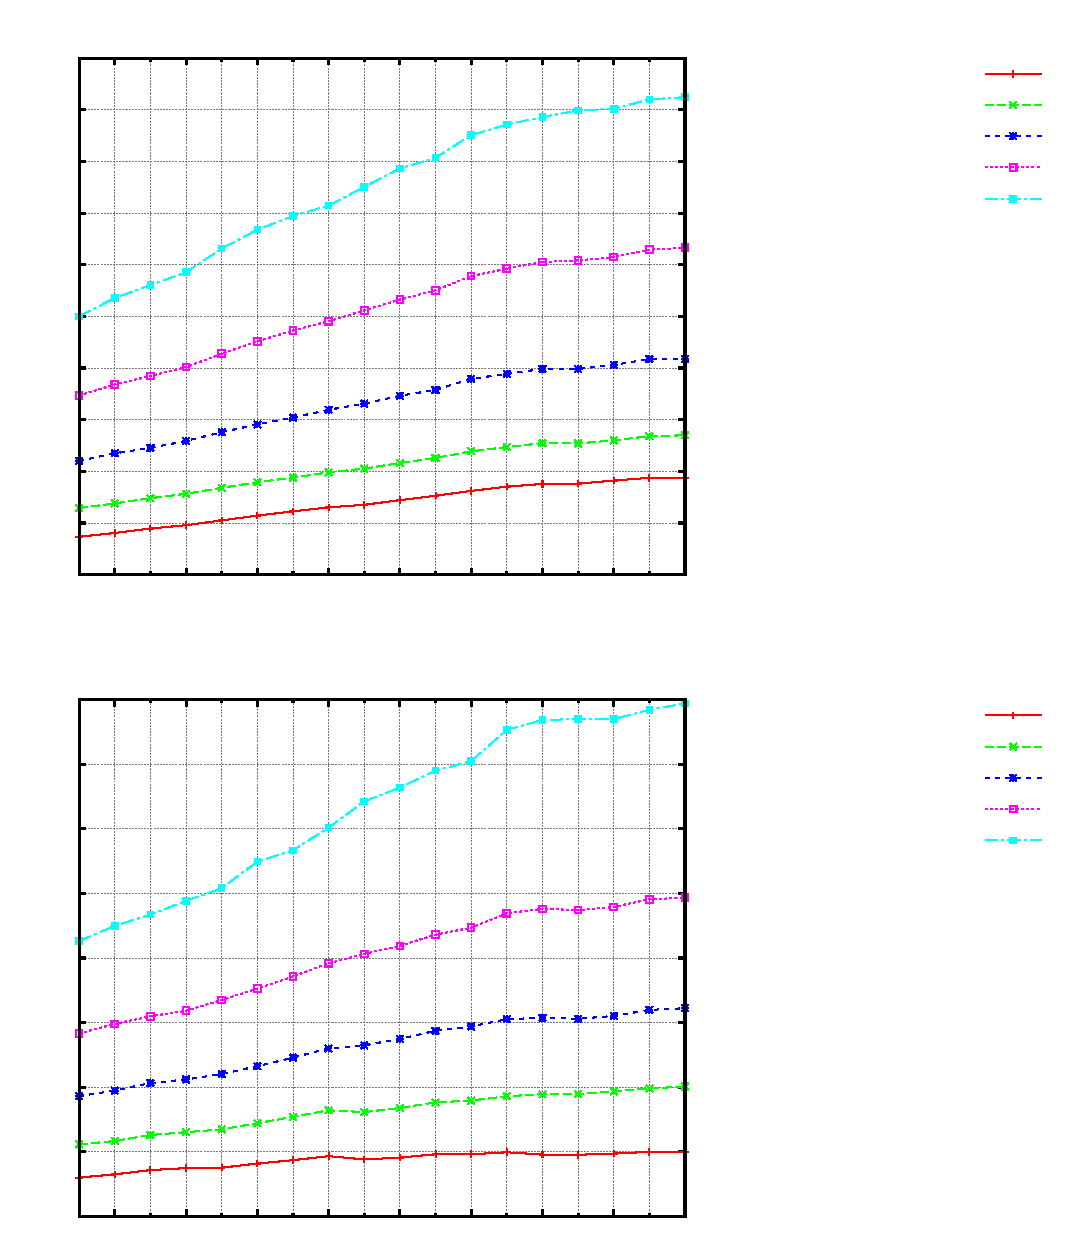
\includegraphics{./plots/wage-percentiles-ftpt/wage-percentiles.eps}}%
    \gplfronttext
  \end{picture}%
\endgroup
